% CVPR 2022 Paper Template
% based on the CVPR template provided by Ming-Ming Cheng (https://github.com/MCG-NKU/CVPR_Template)
% modified and extended by Stefan Roth (stefan.roth@NOSPAMtu-darmstadt.de)

\documentclass[10pt,twocolumn,letterpaper]{article}

%%%%%%%%% PAPER TYPE  - PLEASE UPDATE FOR FINAL VERSION
% \usepackage[review]{cvpr}      % To produce the REVIEW version
\usepackage{cvpr}              % To produce the CAMERA-READY version
%\usepackage[pagenumbers]{cvpr} % To force page numbers, e.g. for an arXiv version

% Include other packages here, before hyperref.
\usepackage{graphicx}
\graphicspath{ {./image/} }
\usepackage{caption}
\usepackage{subcaption}
\usepackage{graphicx}
\usepackage{amsmath}
\usepackage{amssymb}
\usepackage{booktabs}

% It is strongly recommended to use hyperref, especially for the review version.
% hyperref with option pagebackref eases the reviewers' job.
% Please disable hyperref *only* if you encounter grave issues, e.g. with the
% file validation for the camera-ready version.
%
% If you comment hyperref and then uncomment it, you should delete
% ReviewTempalte.aux before re-running LaTeX.
% (Or just hit 'q' on the first LaTeX run, let it finish, and you
%  should be clear).
\usepackage[pagebackref,breaklinks,colorlinks]{hyperref}


% Support for easy cross-referencing
\usepackage[capitalize]{cleveref}
\crefname{section}{Sec.}{Secs.}
\Crefname{section}{Section}{Sections}
\Crefname{table}{Table}{Tables}
\crefname{table}{Tab.}{Tabs.}


%%%%%%%%% PAPER ID  - PLEASE UPDATE
\def\cvprPaperID{918299101} % *** Enter the CVPR Paper ID here
\def\confName{CVPR}
\def\confYear{2023}

\begin{document}

%%%%%%%%% TITLE - PLEASE UPDATE
\title{Acquiring, Processing, and Displaying JWST NIRCam Imaging Data}
\cvprfinaltrue

\author{Maxwell Oakes\\
Portland State University\\
1900 SW 4th Ave, Portland, OR 97201\\
{\tt\small maxoakes@pdx.edu}}
\maketitle

%%%%%%%%% ABSTRACT
\begin{abstract}
  Images coming back from the James Webb Space Telescope (JWST) present a fascinating and awe-inspiring look at distant celestial objects and provide a glimpse at the early history of the universe. 
  This paper provides a summary of steps taken to replicate the work done to process raw astronomical imaging data into the vivid RGB images that have been released by The National Aeronautics and Space Administration (NASA). 
  Methods to acquire the image files via download will be addressed, as well as an overview of the FITS file format in which they are contained.
  The steps required to contextualize and realign the images will also be reviewed. A short description of any post-processing steps will be provided before a discussion of the results that were obtained.
  The processed images that have been released from JWST were placed into an already-existing processing pipeline managed by developers and graphics artists that have already spent much time in the field, so the results of this project will not be at the expert-level quality of those images, but the general process described may shed light on how steps of that process is done.
\end{abstract}

%%%%%%%%% BODY TEXT
\section{Introduction}
\label{sec:intro}

The James Webb Space Telescope (JWST) was launched December 25th, 2021 as a successor to Hubble Space Telescope. The mission for JWST is to examine every phase of cosmic history; ranging from the first stars after the Big Bang to the formation of galaxies, stars and planets. Of the goals for JWST, there are four themes: 
(1) peer back in time with infrared imaging to see the formation of the first stars and galaxies, 
(2) use highly-sensitive infrared technology to view faint and early galaxies to help us understand how they are formed,
(3) see through clouds of dust and gas to observe how planetary systems are born
(4) study atmospheres of extrasolar planets in hopes of finding the building blocks of life elsewhere in the universe \cite{webbobjective}.
Altogether, these objectives aim to give humanity a better understanding of the universe and its formation, and help us better understand our place in the universe.

Being able to meaningfully process data from JWST will prove to be immensely important in achieving these objectives. Additionally, allowing the public audience to see the fruits of JWST will drive fascination, and perhaps garner support in its ultimate objective.

Currently, the publishing of images from JWST's NIRCam imager requires a mix of computer science and art to achieve eye-catching imagery, often requiring external photo editing software and subjective judgement to make the best decisions.

This project aims to streamline the post-processing step of NIRCam data by automatically downloading imaging data from Space Telescope Science Institute's (STSI) MAST public archive, select the best wavelength-filtered exposures and combine them into a single correctly-aligned, clean RGB color image.

\section{Background Information}
\label{sec:background}

The following offers a short description of JWST and its instruments and capabilities, and gives a summary of the processing pipeline of imaging data, and concludes with the basic data structure that this imaging data comes in.

\subsection{Onboard Instruments}

\begin{figure*}
  \centering
    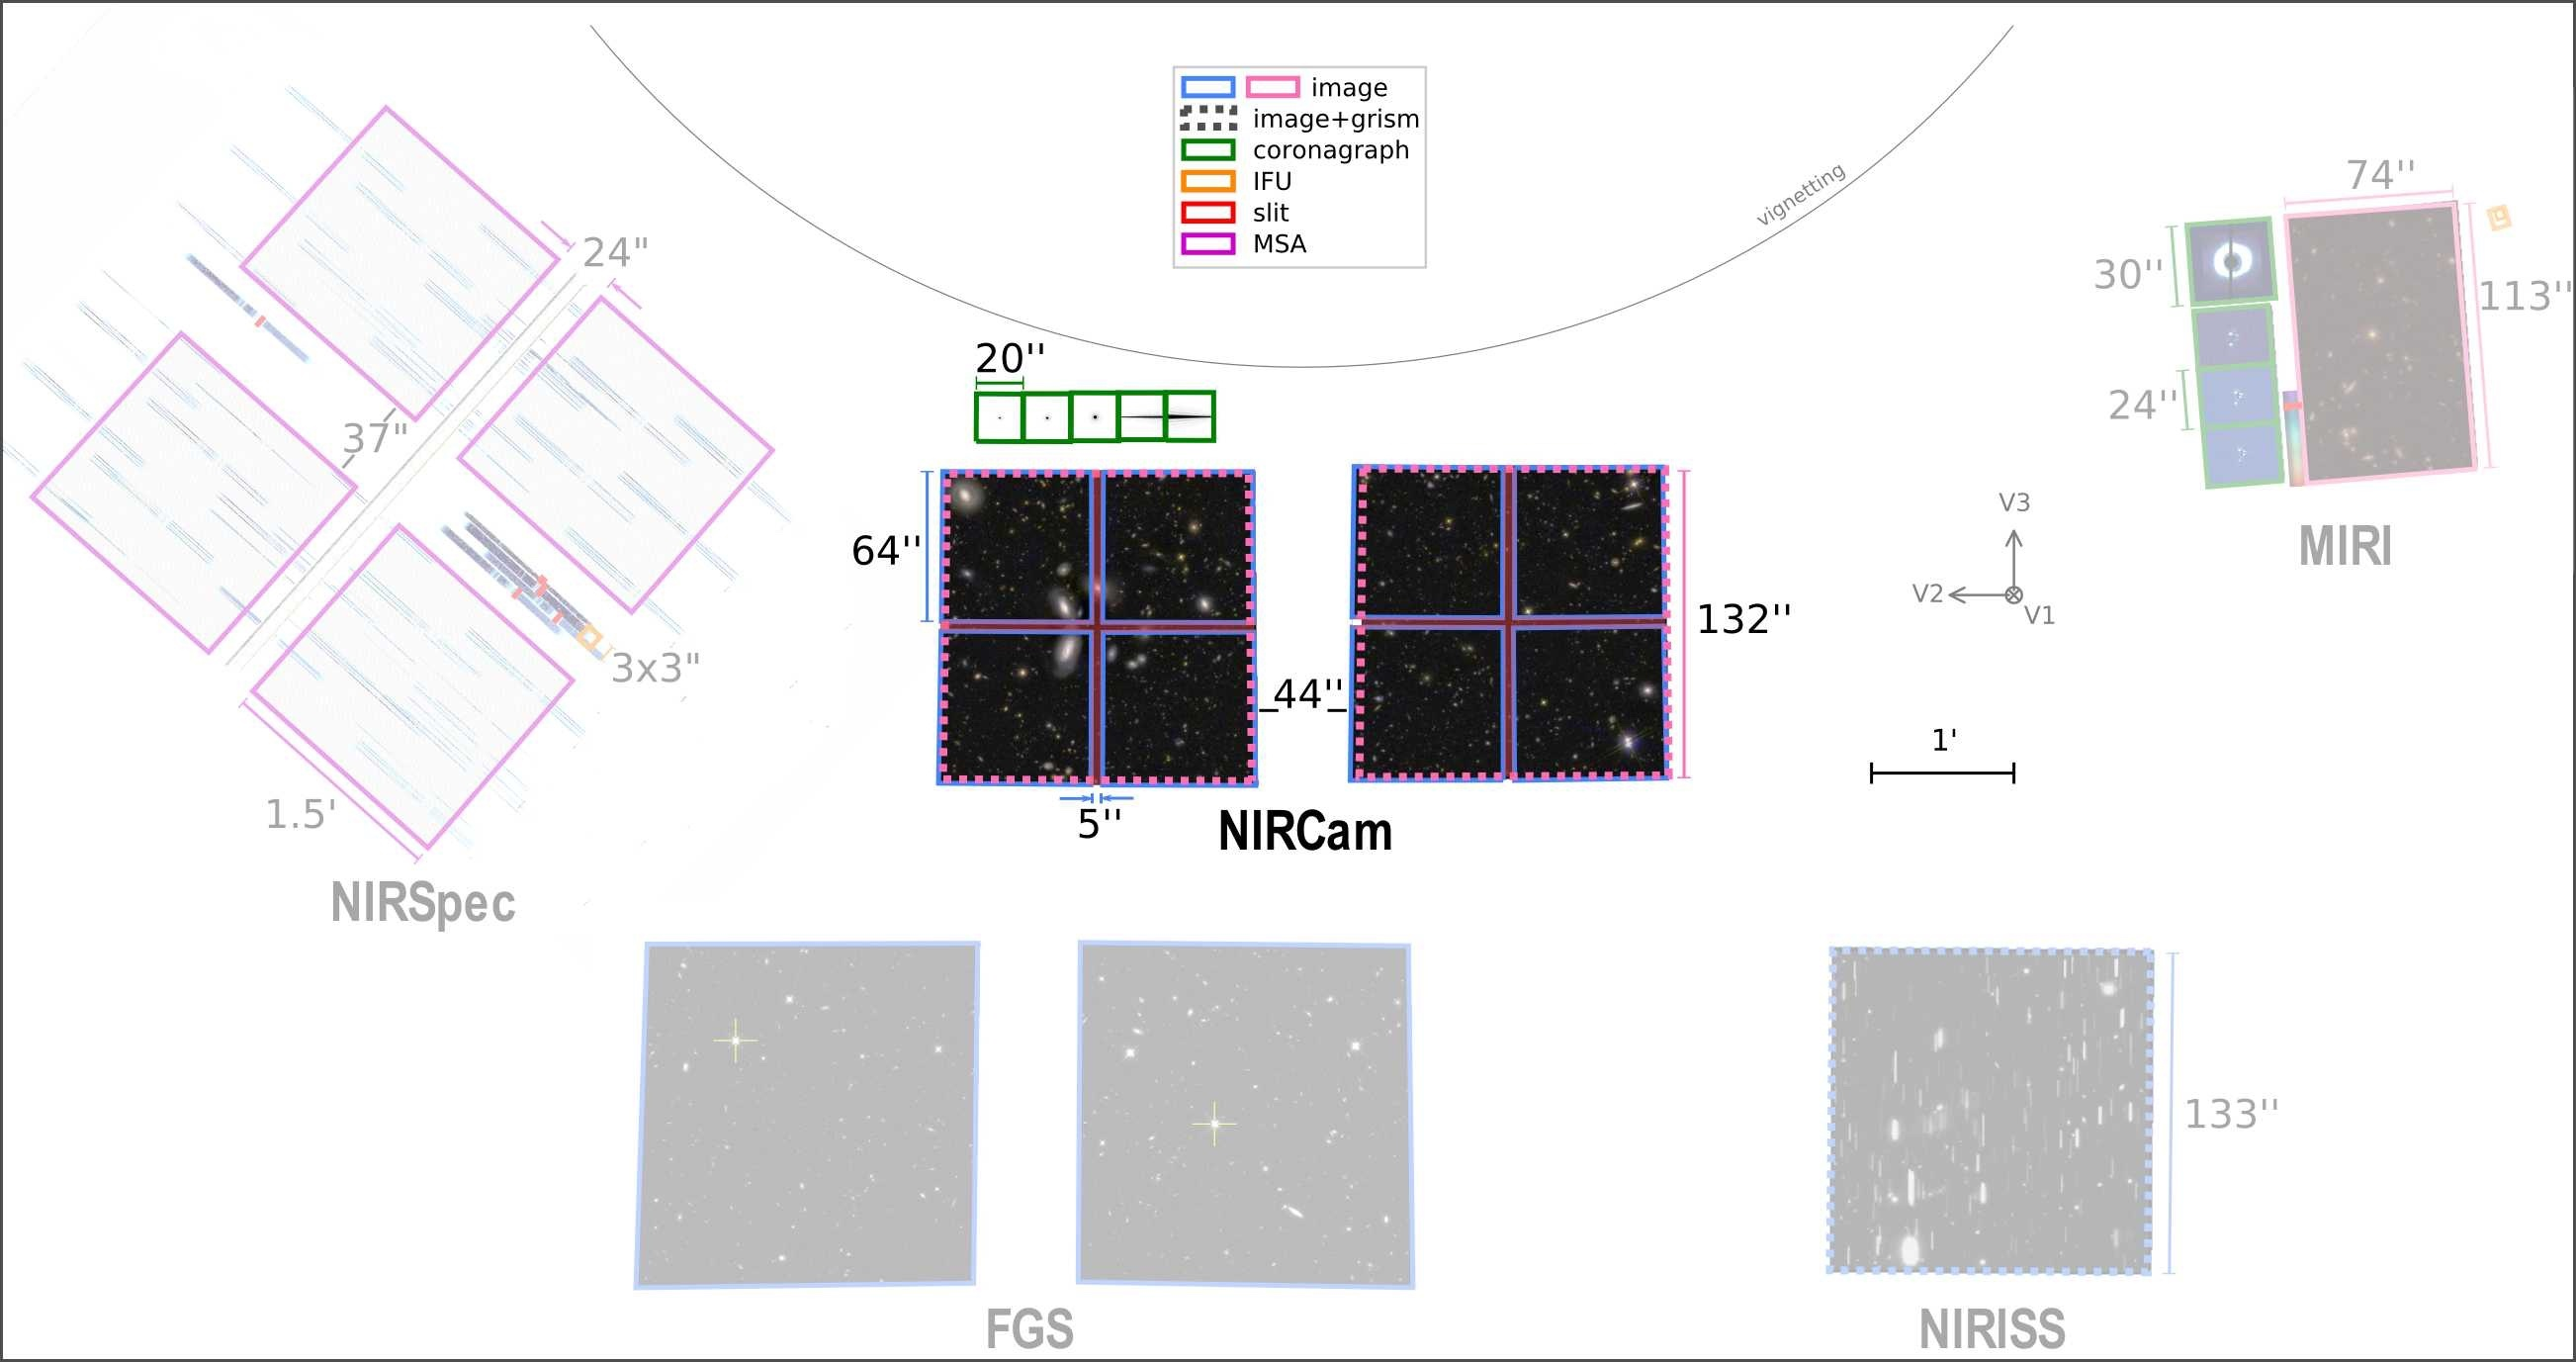
\includegraphics[scale=0.18]{instrument_array}
  \caption{Placement of instrument array onboard JWST \cite{webbnircam}. The instrument that is focused is NIRCam, the primary tool that will be used in the project presented in this paper.}
  \label{fig:instruments}
\end{figure*}

In order to achieve these objectives, JWST is armed with several imaging and spectroscopy tools described below, and shown in \cref{fig:instruments}:
\newline

\textbf{MIRI Imager:} A camera sensor able to capture between $5.6$ and $25.5\mu m$. It offers 9 broadband filters allowing the capture of smaller portions of this light bandwidth. 
The camera itself has a field of view of $74'' \times 113''$. It also features several dither patterns that improve sampling at the shorter wavelengths, and remove artifacts from the detector or cosmic ray hits \cite{webbmiri}.
\newline

\textbf{NIRCam Infrared Camera:} A tool that offers many observation modes from regular imaging to coronagraphic imaging, to wide field slitless spectroscopy. For this project, NIRCam will be the primary instrument that is studied and utilized.
For imaging, NIRCam has two $2.2' \times 2.2'$ fields that cover $9.7$ arcmin$^2$ with a total of 29 available wavelength filters.
The coronagraphic imaging mode offers occlusion masks offer round bar-shaped occulting masks allowing for the capture of a star's corona without capturing the intense light of the star's center \cite{webbnircam}. In some of the pre-processed images of this project, some of the larger stars will have occlusion masks featured in the image outputs.
\newline

\textbf{NIRISS Imaging:} An imager that enables capture of wavelengths between $0.8$ and $5.0\mu m$ in a $2.2' \times 2.2'$ field of view. 
Like NIRCam, NIRISS offers spectroscopy, but it is more sensitive to low surface brightness between $0.8$ and $2.5\mu m$. 
NIRISS imaging is also an alternative to NIRCam in cases where the position of a target is not known with great accuracy \cite{webbniriss}.
\newline

\textbf{NIRSPEC Spectroscopy:} Provides near-IR spectroscopy between $0.6$ and $5.3 \mu m$ in a $3.4 \times 3.6$ arcmin field of view. It is designed to be especially powerful for multiplexing spectroscopy and high contrast high throughput single-object spectroscopy \cite{webbnirspec}.

\subsection{Filters}

\begin{figure}[t]
  \centering
  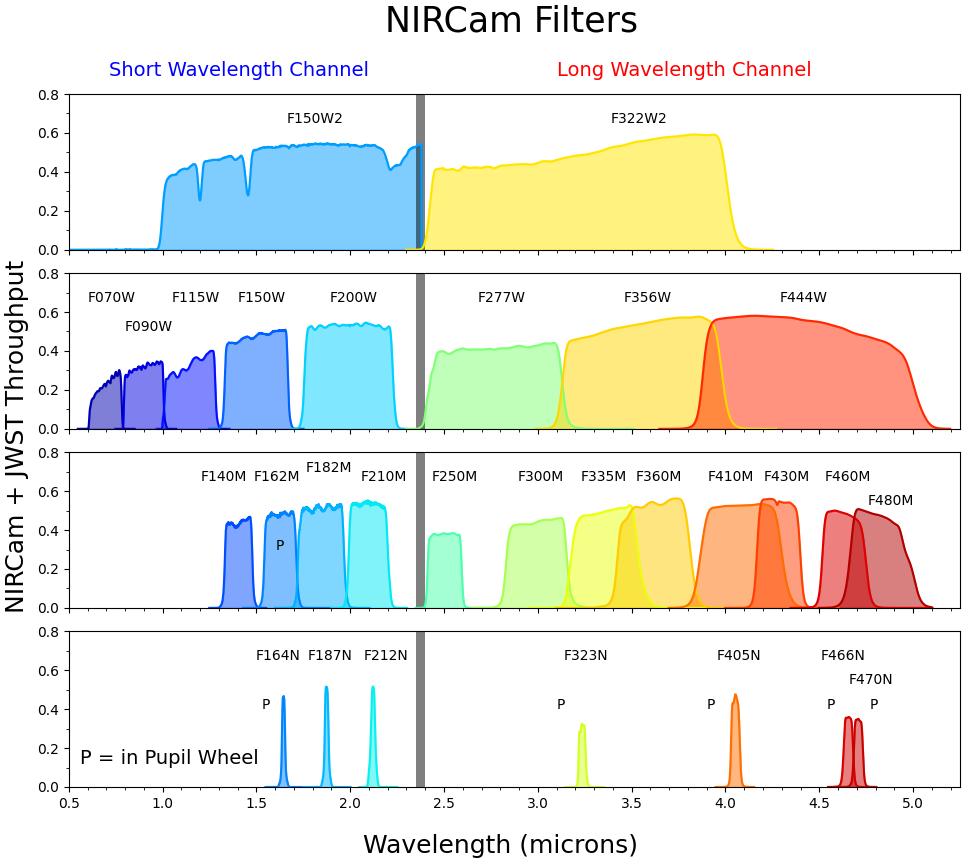
\includegraphics[scale=0.33]{filters}
  \caption{Available filters for the NIRCam instrument. Those marked with (P) are on the pupil wheel which require transmission through a second filter on the filter wheel \cite{webbfilters}.}
  \label{fig:filters}
\end{figure}

JWST is able to capture between $0.6 -- 28.8\mu m$ between all available tools. On each instrument, there are several filters that allow for capturing a smaller bandwidth of that total.
On NIRCam alone, there are 29 filters available: some for short wavelengths ($0.6-2.3 \mu m$) and some for long wavelengths ($2.4 -- 5.0 \mu m$). Many of these filters can be used in combination of each other by means of a filter wheel and pupil wheel \cite{webbfilters}. 
For this project, the pupil wheel will either be clear (i.e, no filter), or filtering for a wavelength, and the filter wheel will always be set to some wavelength.

\subsection{JWST Data Processing}

The processing of JWST goes through 3 stages. Stage 1 consists of detector-level corrections that are performed on a group-by-group basis. The output of this stage is a countrate image measuring the collection of photons.
Stage 2 includes additional instrument-level corrections to produce fully calibrated image exposures. There are different pipelines for imaging and spectroscopic exposures.
Stage 3 consists of working of with multiple exposures and often consists of combining exposures in some way \cite{webbstages}. 
This is the stage that will primarily be used in the project described by this paper. Stage 3 processing adds corrections for astrometric alignment, background matching of the different mosaics, and outlier rejection \cite{webbstage3}. 
The output of this stage, for NIRCam imaging specifically, are clean and calibrated images with metadata detailing photometry, physical positioning, timing, exposure, and much more.

\subsection{Post-Processing by Astronomers}
When the end goal is to out a color image from NIRCam, it is common that, after stage 3 data processing as previously described, several of the filter exposure images of a mission are compiled in image processing software like Photoshop \cite{editinterview}. At this point, it is up to the graphics artist to interpret the exposures and try to output the most visually striking combination of filters using only three color channels.

\subsection{FITS File Format}
FITS files are the only format that house JWST (and most astronomical) data. They consist of one or more Header + Data Units (HDUs). 
Each HDU can contain a table data structure that resembles a dictionary, but rather than a key and a value, this table contains a keyword, value, and comment. Each element in this table type is called a 'card'. 
An HDU can also contain an N-dimensional array, frequently a 1D spectrum, 2D image, or 3D data cube. The values in this array can be integers (signed, or unsigned for 8-bit), or floats of varying sizes. \cite{fitsdoc}

In the context of JWST stage 3 data used in this project, it is very common that a FITS file contains a primary HDU that has no array and a table with upwards of 300+ cards with information about the mission, target object, and previous stage's processing steps.

Alongside the primary HDU exists the 'science' HDU that contains the raw exposure data for the captured filtered wavelength. The accompanying table of cards is a lot shorter and contains information regarding the applied filter(s), exposure time, spacecraft orientation, spatial extent, as well as other metadata pertinent to the capture of the image.

There are several other HDUs in the FITS file, most of which measure uncertainty and variance for each pixel in the 'science' HDU array \cite{webbfits}. The remaining HDUs are not relevant to processing of the image data. 

\subsection{MAST Archive}

\subsection{Astropy and Python}

\section{Methodology}
\label{sec:script}
\subsection{Data Acquisition}
\subsection{Image Processing}
\subsection{Image Display}

\section{Experiments}
\label{sec:exp}

\section{Discussion}
\label{sec:disc}

%-------------------------------------------------------------------------
\section{Junk}
\label{sec:xxx}

\subsection{The ruler}
The \LaTeX\ style defines a printed ruler which should be present in the version submitted for review.
The ruler is provided in order that reviewers may comment on particular lines in the paper without circumlocution.
If you are preparing a document using a non-\LaTeX\ document preparation system, please arrange for an equivalent ruler to appear on the final output pages.
The presence or absence of the ruler should not change the appearance of any other content on the page.
The camera-ready copy should not contain a ruler.
(\LaTeX\ users may use options of cvpr.sty to switch between different versions.)

Reviewers:
note that the ruler measurements do not align well with lines in the paper --- this turns out to be very difficult to do well when the paper contains many figures and equations, and, when done, looks ugly.
Just use fractional references (\eg, this line is $087.5$), although in most cases one would expect that the approximate location will be adequate.


\subsection{Paper ID}
Make sure that the Paper ID from the submission system is visible in the version submitted for review (replacing the ``*****'' you see in this document).
If you are using the \LaTeX\ template, \textbf{make sure to update paper ID in the appropriate place in the tex file}.


\subsection{Mathematics}

Please number all of your sections and displayed equations as in these examples:
\begin{equation}
  E = m\cdot c^2
  \label{eq:important}
\end{equation}
and
\begin{equation}
  v = a\cdot t.
  \label{eq:also-important}
\end{equation}
It is important for readers to be able to refer to any particular equation.
Just because you did not refer to it in the text does not mean some future reader might not need to refer to it.
It is cumbersome to have to use circumlocutions like ``the equation second from the top of page 3 column 1''.
(Note that the ruler will not be present in the final copy, so is not an alternative to equation numbers).
All authors will benefit from reading Mermin's description of how to write mathematics:
\url{http://www.pamitc.org/documents/mermin.pdf}.

\subsection{Blind review}

Many authors misunderstand the concept of anonymizing for blind review.
Blind review does not mean that one must remove citations to one's own work---in fact it is often impossible to review a paper unless the previous citations are known and available.

Blind review means that you do not use the words ``my'' or ``our'' when citing previous work.
That is all.
(But see below for tech reports.)

Saying ``this builds on the work of Lucy Smith [1]'' does not say that you are Lucy Smith;
it says that you are building on her work.
If you are Smith and Jones, do not say ``as we show in [7]'', say ``as Smith and Jones show in [7]'' and at the end of the paper, include reference 7 as you would any other cited work.

An example of a bad paper just asking to be rejected:
\begin{quote}
\begin{center}
    An analysis of the frobnicatable foo filter.
\end{center}

   In this paper we present a performance analysis of our previous paper [1], and show it to be inferior to all previously known methods.
   Why the previous paper was accepted without this analysis is beyond me.

   [1] Removed for blind review
\end{quote}


An example of an acceptable paper:
\begin{quote}
\begin{center}
     An analysis of the frobnicatable foo filter.
\end{center}

   In this paper we present a performance analysis of the  paper of Smith \etal [1], and show it to be inferior to all previously known methods.
   Why the previous paper was accepted without this analysis is beyond me.

   [1] Smith, L and Jones, C. ``The frobnicatable foo filter, a fundamental contribution to human knowledge''. Nature 381(12), 1-213.
\end{quote}

If you are making a submission to another conference at the same time, which covers similar or overlapping material, you may need to refer to that submission in order to explain the differences, just as you would if you had previously published related work.
In such cases, include the anonymized parallel submission~\cite{Authors14} as supplemental material and cite it as
\begin{quote}
[1] Authors. ``The frobnicatable foo filter'', F\&G 2014 Submission ID 324, Supplied as supplemental material {\tt fg324.pdf}.
\end{quote}

Finally, you may feel you need to tell the reader that more details can be found elsewhere, and refer them to a technical report.
For conference submissions, the paper must stand on its own, and not {\em require} the reviewer to go to a tech report for further details.
Thus, you may say in the body of the paper ``further details may be found in~\cite{Authors14b}''.
Then submit the tech report as supplemental material.
Again, you may not assume the reviewers will read this material.

Sometimes your paper is about a problem which you tested using a tool that is widely known to be restricted to a single institution.
For example, let's say it's 1969, you have solved a key problem on the Apollo lander, and you believe that the CVPR70 audience would like to hear about your
solution.
The work is a development of your celebrated 1968 paper entitled ``Zero-g frobnication: How being the only people in the world with access to the Apollo lander source code makes us a wow at parties'', by Zeus \etal.

You can handle this paper like any other.
Do not write ``We show how to improve our previous work [Anonymous, 1968].
This time we tested the algorithm on a lunar lander [name of lander removed for blind review]''.
That would be silly, and would immediately identify the authors.
Instead write the following:
\begin{quotation}
\noindent
   We describe a system for zero-g frobnication.
   This system is new because it handles the following cases:
   A, B.  Previous systems [Zeus et al. 1968] did not  handle case B properly.
   Ours handles it by including a foo term in the bar integral.

   ...

   The proposed system was integrated with the Apollo lunar lander, and went all the way to the moon, don't you know.
   It displayed the following behaviours, which show how well we solved cases A and B: ...
\end{quotation}
As you can see, the above text follows standard scientific convention, reads better than the first version, and does not explicitly name you as the authors.
A reviewer might think it likely that the new paper was written by Zeus \etal, but cannot make any decision based on that guess.
He or she would have to be sure that no other authors could have been contracted to solve problem B.
\medskip

\noindent
FAQ\medskip\\
{\bf Q:} Are acknowledgements OK?\\
{\bf A:} No.  Leave them for the final copy.\medskip\\
{\bf Q:} How do I cite my results reported in open challenges?
{\bf A:} To conform with the double-blind review policy, you can report results of other challenge participants together with your results in your paper.
For your results, however, you should not identify yourself and should not mention your participation in the challenge.
Instead present your results referring to the method proposed in your paper and draw conclusions based on the experimental comparison to other results.\medskip\\

\begin{figure}[t]
  \centering
  \fbox{\rule{0pt}{2in} \rule{0.9\linewidth}{0pt}}
   %\includegraphics[width=0.8\linewidth]{egfigure.eps}

   \caption{Example of caption.
   It is set in Roman so that mathematics (always set in Roman: $B \sin A = A \sin B$) may be included without an ugly clash.}
   \label{fig:onecol}
\end{figure}

\subsection{Miscellaneous}

\noindent
Compare the following:\\
\begin{tabular}{ll}
 \verb'$conf_a$' &  $conf_a$ \\
 \verb'$\mathit{conf}_a$' & $\mathit{conf}_a$
\end{tabular}\\
See The \TeX book, p165.

The space after \eg, meaning ``for example'', should not be a sentence-ending space.
So \eg is correct, {\em e.g.} is not.
The provided \verb'\eg' macro takes care of this.

When citing a multi-author paper, you may save space by using ``et alia'', shortened to ``\etal'' (not ``{\em et.\ al.}'' as ``{\em et}'' is a complete word).
If you use the \verb'\etal' macro provided, then you need not worry about double periods when used at the end of a sentence as in Alpher \etal.
However, use it only when there are three or more authors.
Thus, the following is correct:
   ``Frobnication has been trendy lately.
   It was introduced by Alpher~\cite{Alpher02}, and subsequently developed by
   Alpher and Fotheringham-Smythe~\cite{Alpher03}, and Alpher \etal~\cite{Alpher04}.''

This is incorrect: ``... subsequently developed by Alpher \etal~\cite{Alpher03} ...'' because reference~\cite{Alpher03} has just two authors.


% Update the cvpr.cls to do the following automatically.
% For this citation style, keep multiple citations in numerical (not
% chronological) order, so prefer \cite{Alpher03,Alpher02,Authors14} to
% \cite{Alpher02,Alpher03,Authors14}.


\begin{figure*}
  \centering
  \begin{subfigure}{0.5\linewidth}
    \fbox{\rule{0pt}{2in} \rule{.9\linewidth}{0pt}}
    \caption{An example of a subfigure.}
    \label{fig:short-a}
  \end{subfigure}
  \hfill
  \begin{subfigure}{0.4\linewidth}
    \fbox{\rule{0pt}{2in} \rule{.9\linewidth}{0pt}}
    \caption{Another example.}
    \label{fig:short-b}
  \end{subfigure}
  \caption{Example of a short caption, which should be centered.}
  \label{fig:short}
\end{figure*}

%------------------------------------------------------------------------
\section{Formatting your paper}
\label{sec:formatting}

All text must be in a two-column format.
The total allowable size of the text area is $6\frac78$ inches (17.46 cm) wide by $8\frac78$ inches (22.54 cm) high.
Columns are to be $3\frac14$ inches (8.25 cm) wide, with a $\frac{5}{16}$ inch (0.8 cm) space between them.
The main title (on the first page) should begin 1 inch (2.54 cm) from the top edge of the page.
The second and following pages should begin 1 inch (2.54 cm) from the top edge.
On all pages, the bottom margin should be $1\frac{1}{8}$ inches (2.86 cm) from the bottom edge of the page for $8.5 \times 11$-inch paper;
for A4 paper, approximately $1\frac{5}{8}$ inches (4.13 cm) from the bottom edge of the
page.

%-------------------------------------------------------------------------
\subsection{Margins and page numbering}

All printed material, including text, illustrations, and charts, must be kept
within a print area $6\frac{7}{8}$ inches (17.46 cm) wide by $8\frac{7}{8}$ inches (22.54 cm)
high.
%
Page numbers should be in the footer, centered and $\frac{3}{4}$ inches from the bottom of the page.
The review version should have page numbers, yet the final version submitted as camera ready should not show any page numbers.
The \LaTeX\ template takes care of this when used properly.



%-------------------------------------------------------------------------
\subsection{Type style and fonts}

Wherever Times is specified, Times Roman may also be used.
If neither is available on your word processor, please use the font closest in
appearance to Times to which you have access.

MAIN TITLE.
Center the title $1\frac{3}{8}$ inches (3.49 cm) from the top edge of the first page.
The title should be in Times 14-point, boldface type.
Capitalize the first letter of nouns, pronouns, verbs, adjectives, and adverbs;
do not capitalize articles, coordinate conjunctions, or prepositions (unless the title begins with such a word).
Leave two blank lines after the title.

AUTHOR NAME(s) and AFFILIATION(s) are to be centered beneath the title
and printed in Times 12-point, non-boldface type.
This information is to be followed by two blank lines.

The ABSTRACT and MAIN TEXT are to be in a two-column format.

MAIN TEXT.
Type main text in 10-point Times, single-spaced.
Do NOT use double-spacing.
All paragraphs should be indented 1 pica (approx.~$\frac{1}{6}$ inch or 0.422 cm).
Make sure your text is fully justified---that is, flush left and flush right.
Please do not place any additional blank lines between paragraphs.

Figure and table captions should be 9-point Roman type as in \cref{fig:onecol,fig:short}.
Short captions should be centred.

\noindent Callouts should be 9-point Helvetica, non-boldface type.
Initially capitalize only the first word of section titles and first-, second-, and third-order headings.

FIRST-ORDER HEADINGS.
(For example, {\large \bf 1. Introduction}) should be Times 12-point boldface, initially capitalized, flush left, with one blank line before, and one blank line after.

SECOND-ORDER HEADINGS.
(For example, { \bf 1.1. Database elements}) should be Times 11-point boldface, initially capitalized, flush left, with one blank line before, and one after.
If you require a third-order heading (we discourage it), use 10-point Times, boldface, initially capitalized, flush left, preceded by one blank line, followed by a period and your text on the same line.

%-------------------------------------------------------------------------
\subsection{Footnotes}

Please use footnotes\footnote{This is what a footnote looks like.
It often distracts the reader from the main flow of the argument.} sparingly.
Indeed, try to avoid footnotes altogether and include necessary peripheral observations in the text (within parentheses, if you prefer, as in this sentence).
If you wish to use a footnote, place it at the bottom of the column on the page on which it is referenced.
Use Times 8-point type, single-spaced.


%-------------------------------------------------------------------------
\subsection{Cross-references}

For the benefit of author(s) and readers, please use the
{\small\begin{verbatim}
  \cref{...}
\end{verbatim}}  command for cross-referencing to figures, tables, equations, or sections.
This will automatically insert the appropriate label alongside the cross-reference as in this example:
\begin{quotation}
  To see how our method outperforms previous work, please see \cref{fig:onecol} and \cref{tab:example}.
  It is also possible to refer to multiple targets as once, \eg~to \cref{fig:onecol,fig:short-a}.
  You may also return to \cref{sec:formatting} or look at \cref{eq:also-important}.
\end{quotation}
If you do not wish to abbreviate the label, for example at the beginning of the sentence, you can use the
{\small\begin{verbatim}
  \Cref{...}
\end{verbatim}}
command. Here is an example:
\begin{quotation}
  \Cref{fig:onecol} is also quite important.
\end{quotation}

%-------------------------------------------------------------------------
\subsection{References}

List and number all bibliographical references in 9-point Times, single-spaced, at the end of your paper.
When referenced in the text, enclose the citation number in square brackets, for
example~\cite{Authors14}.
Where appropriate, include page numbers and the name(s) of editors of referenced books.
When you cite multiple papers at once, please make sure that you cite them in numerical order like this \cite{Alpher02,Alpher03,Alpher05,Authors14b,Authors14}.
If you use the template as advised, this will be taken care of automatically.

\begin{table}
  \centering
  \begin{tabular}{@{}lc@{}}
    \toprule
    Method & Frobnability \\
    \midrule
    Theirs & Frumpy \\
    Yours & Frobbly \\
    Ours & Makes one's heart Frob\\
    \bottomrule
  \end{tabular}
  \caption{Results.   Ours is better.}
  \label{tab:example}
\end{table}

%-------------------------------------------------------------------------
\subsection{Illustrations, graphs, and photographs}

All graphics should be centered.
In \LaTeX, avoid using the \texttt{center} environment for this purpose, as this adds potentially unwanted whitespace.
Instead use
{\small\begin{verbatim}
  \centering
\end{verbatim}}
at the beginning of your figure.
Please ensure that any point you wish to make is resolvable in a printed copy of the paper.
Resize fonts in figures to match the font in the body text, and choose line widths that render effectively in print.
Readers (and reviewers), even of an electronic copy, may choose to print your paper in order to read it.
You cannot insist that they do otherwise, and therefore must not assume that they can zoom in to see tiny details on a graphic.

When placing figures in \LaTeX, it's almost always best to use \verb+\includegraphics+, and to specify the figure width as a multiple of the line width as in the example below
{\small\begin{verbatim}
   \usepackage{graphicx} ...
   \includegraphics[width=0.8\linewidth]
                   {myfile.pdf}
\end{verbatim}
}


%-------------------------------------------------------------------------
\subsection{Color}

Please refer to the author guidelines on the \confName\ \confYear\ web page for a discussion of the use of color in your document.

If you use color in your plots, please keep in mind that a significant subset of reviewers and readers may have a color vision deficiency; red-green blindness is the most frequent kind.
Hence avoid relying only on color as the discriminative feature in plots (such as red \vs green lines), but add a second discriminative feature to ease disambiguation.

%------------------------------------------------------------------------
\section{Final copy}

You must include your signed IEEE copyright release form when you submit your finished paper.
We MUST have this form before your paper can be published in the proceedings.

Please direct any questions to the production editor in charge of these proceedings at the IEEE Computer Society Press:
\url{https://www.computer.org/about/contact}.

\LaTeX{} \cite{lamport94} is a set of macros built atop \TeX{} \cite{texbook}.
%%%%%%%%% REFERENCES
\begin{thebibliography}{9}
\bibitem{webbobjective}
$https://www.nasa.gov/mission_pages/webb/science/index.html$

\bibitem{webbtools}
$https://archive.stsci.edu/missions-and-data/jwst$

\bibitem{webbmiri}
$https://jwst-docs.stsci.edu/jwst-mid-infrared-instrument/miri-observing-modes/miri-imaging$

\bibitem{webbnircam}
$https://jwst-docs.stsci.edu/jwst-near-infrared-camera$

\bibitem{webbniriss}
$https://jwst-docs.stsci.edu/jwst-near-infrared-imager-and-slitless-spectrograph/niriss-observing-modes/niriss-imaging$

\bibitem{webbnirspec}
$https://jwst-docs.stsci.edu/jwst-near-infrared-spectrograph$

\bibitem{webbfilters}
$https://jwst-docs.stsci.edu/jwst-near-infrared-camera/nircam-instrumentation/nircam-filters$

\bibitem{webbstages}
$https://jwst-pipeline.readthedocs.io/en/stable/jwst/pipeline/main.html$

\bibitem{webbstage3}
$https://jwst-pipeline.readthedocs.io/en/stable/jwst/pipeline/calwebb_image3.html\#calwebb-image3$

\bibitem{editinterview}
$https://www.space.com/james-webb-space-telescope-image-editing$

\bibitem{fitsdoc}
$https://www.loc.gov/preservation/digital/formats/fdd/fdd000317.shtml$

\bibitem{webbfits}
$https://jwst-pipeline.readthedocs.io/en/stable/jwst/data_products/science_products.html\#resampled-2-d-data-i2d-and-s2d$
\end{thebibliography}

\end{document}